%
% Setup
\chapter{System setup and control algorithm}

As explained in the introduction, the control of the algorithm is centralized, therefore a single agent controls the whole system. A \ac{MCS} is used to determine the position and attitude of the drones.

\label{chap::setup}
\section{Hardware and properties}
This is the hardware used in the thesis:
\setitemize{itemsep=-5pt}
\begin{itemize}
	\item \ac{MCS} by OptiTrack. The setup consists of 10 cameras filming at around \SI{120}{\hertz}.
	\item 4 Quadcopters (Bebop2 by Parrot, \Cref{fig::bebop}).
	\item 1 Gamepad (Logitech Wireless Gamepad F710, \Cref{fig::gamepad})
	\item Laptop (HP Pavilion 15-au007ns)
	\item Desktop computer (DELL OptiPlex 7050)
\end{itemize}

\begin{figure}
	\centering
	\begin{minipage}{.5\textwidth}
		\centering
		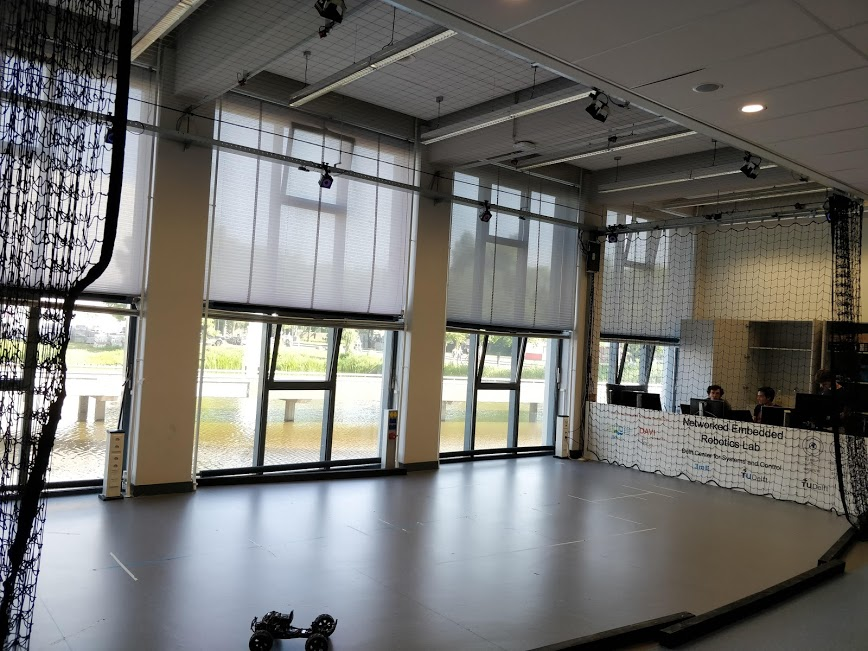
\includegraphics[width=1\linewidth]{Figures/workspace}
		\caption{Drones workspace}
		\label{fig::workspace}
	\end{minipage}%
	\begin{minipage}{.5\textwidth}
		\centering
		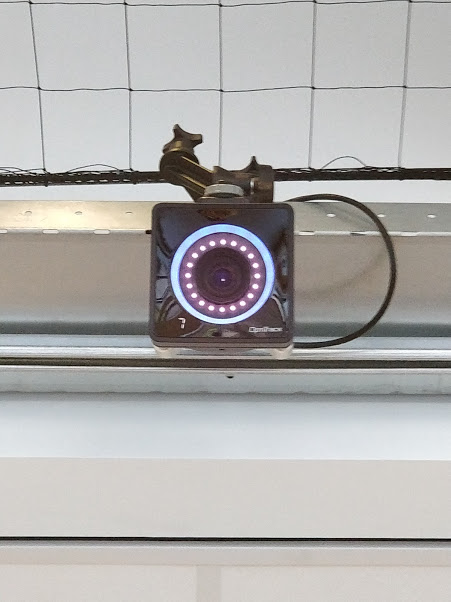
\includegraphics[width=.5\linewidth]{Figures/camera}
		\caption{\ac{MCS} camera}
		\label{fig::camera}
	\end{minipage}
\end{figure}

\begin{figure}
	\centering
	\begin{minipage}{.31\textwidth}
		\centering
		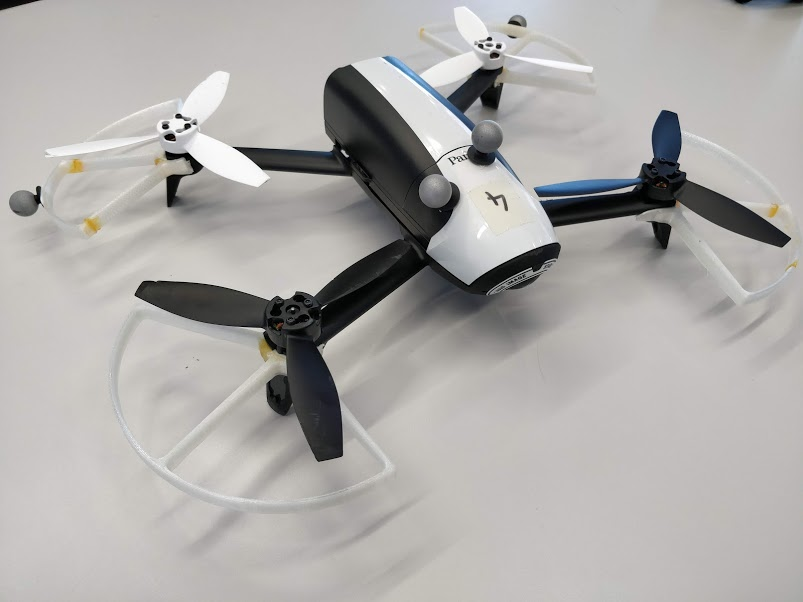
\includegraphics[width=.95\linewidth]{Figures/bebop}
		\caption{Bebop2 drone with markers}
		\label{fig::bebop}
	\end{minipage}%
	\begin{minipage}{.31\textwidth}
		\centering
		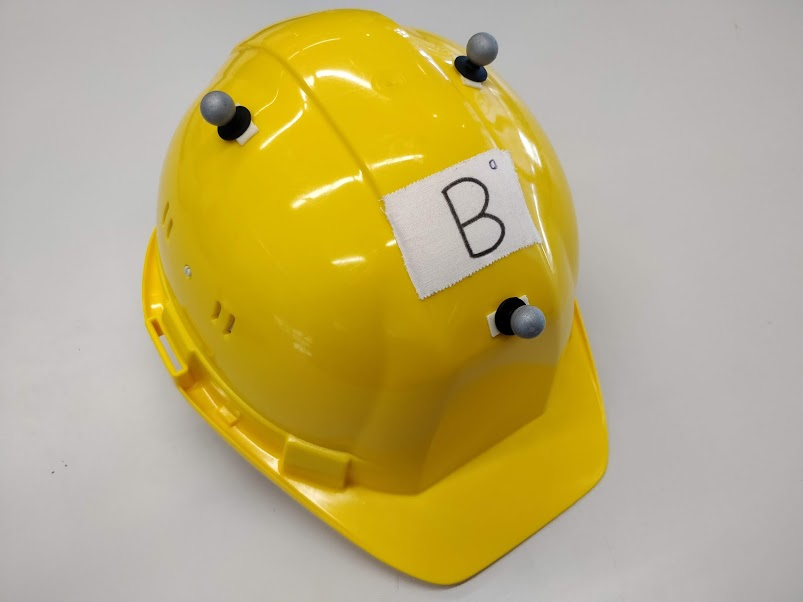
\includegraphics[width=.95\linewidth]{Figures/hat}
		\caption{Hat with reflective markers}
		\label{fig::hat}
	\end{minipage}%
	\begin{minipage}{.31\textwidth}
		\centering
		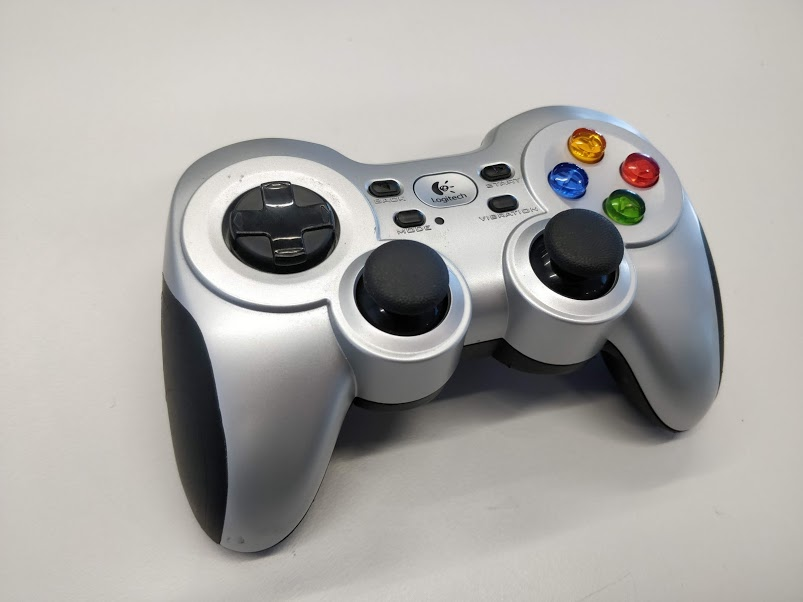
\includegraphics[width=.95\linewidth]{Figures/gamepad}
		\caption{Gamepad by Logitech}
		\label{fig::gamepad}
	\end{minipage}
\end{figure}

\section{Workspace}
The workspace of the drones, seen in  \cref{fig::workspace}, consists on a $6.0\times3.0\times2.6$ \si{\meter} $(L\times W\times H)$ arena where they can move freely while being tracked by the \ac{MCS}. The \ac{MCS} setup consists of 10 cameras such as the one seen in \cref{fig::camera}. The drones, payloads and obstacles are equipped with reflective markers to be tracked by the \ac{MCS}. The markers can be seen in figures \ref{fig::bebop} and \ref{fig::hat}.

\section{Control algorithm}
\label{sect::algorithm}
The basics of the control algorithm will be explained for simulation and the necessary extensions for the experimental setup will be explained in \cref{subsect::experimental_setup} (\nameref{subsect::experimental_setup}).

\subsection{Simulation Algorithm}
We use the following control algorithm: The system starts in a predefined position. Then, using FORCES PRO, a \ac{MPC} plan is generated such as the first stage equals the system state. 

The algorithm assumes that the system follows this plan for one time-step (of $\Delta t$) and calculates the new state using the \ac{EOMs}. The process is then repeated using the new state. A schematic of this solution can be seen in \cref{fig::initial_algorithm}.

During this process, obstacles are also simulated according to predefined movements (that the controller is not aware of).

This data is sent through \ac{ROS} to a visualizer, which will be further explained in \cref{sect::visualizer}


\subsubsection{External Planner}
An additional simulation algorithm was tested and, although it did not prove useful, we will also describe it.

The previous solution has a problem, if the \ac{MPC} solver takes a long time calculating the plan(longer than $1  / \Delta t$ \si{\second}) the simulation will run slower than real time and in the experimental setup the quadrotors will keep repeating the first input for longer than the planner intended. 

This can be solved if we separate the controller from the planner. The planner keeps re-planing using the controller's data as fast as possible, while the controller runs the simulation using inputs from the plan generated by the planner. 

To determine the inputs for each quadrotor, the controller finds the plan’s stage where the drone’s planned position is closest to the actual position. A schematic of this solution can be seen in \cref{fig::external_planner}.

When doing simulated experiments, it was found that cutting the maximum number of iterations of the \ac{MPC} solver in the initial algorithm was better than using an external planner.

\subsection{Initial Solution}
\label{subsect::initial_solution}
When solving the \ac{MPC} problem it is very important to give the solver a good initial solution. To do this we record the previous solution and update it for the next stage. 

If we are using the initial algorithm, the stage will be equal to the second stage in the previous \ac{MPC} solution. Therefore, we can shift the last solution by one stage and add a new stage at the end using the \ac{EOMs}.

\subsubsection{Initial Solution for the External Planner}
The above solution is not suitable for the external planner algorithm as the system could have gone through many stages of the plan.

To do this we compute the path that the controller would follow using the last solution using the same functions that the controller uses to determine the inputs from the plan. 

This initial solution is not good enough and is one of the main causes the external planner algorithm performs worse than the original algorithm.

\subsection{Experimental setup}
\label{subsect::experimental_setup}
As data from the drones tends to be inaccurate (it depends on GPS data and internal assumptions), we will use the \ac{MCS} to determine the position and attitude of the drones. 

A \ac{KF} is used to estimate the state of the system based on the \ac{EOMs} and the data from the \ac{MCS}. \ac{KF} is also used to estimate the location and velocity of the obstacles, which are also tracked with the \ac{MCS}.

\begin{figure}
	\centering
	\begin{minipage}{.5\textwidth}
		\centering
		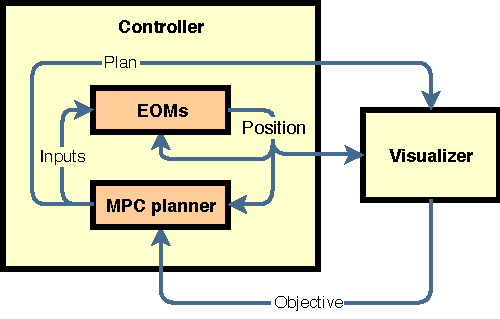
\includegraphics[width=.9\linewidth]{Figures/InitialAlgorithm}
		\caption{Simulation algorithm}
		\label{fig::initial_algorithm}
	\end{minipage}%
	\begin{minipage}{.5\textwidth}
		\centering
		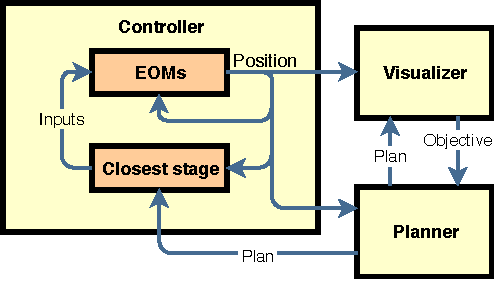
\includegraphics[width=.9\linewidth]{Figures/ExternalPlanner}
		\caption{External planner}
		\label{fig::external_planner}
	\end{minipage}
\end{figure}

\section{Data communication}
\label{sect::communication}
All data goes through the \ac{ROS} network, this means that we can separate different tasks throughout several computers and increase performance. The tasks are:
\begin{itemize}
	\item \textbf{\ac{ROS} core}: One of the computers has to start the \ac{ROS} core, this is a node that manages all communications through the \ac{ROS} network.
	\item \textbf{\ac{MCS} data}: Motive, a proprietary software by OptiTrack, computes the 3D location of the objects based on their markers. This data is then translated by a ROS node and fed to the ROS network.
	\item \textbf{Gamepad input}: A gamepad is connected to one computer through Bluetooth. A \ac{ROS} node in the same computer feeds the controller inputs to the \ac{ROS} network. The gamepad lets the user control the drones manually before turning on \ac{MPC}.
	\item \textbf{Drone commands}: Bebop2 drones create their own wireless network in order to communicate with other hardware. For each drone, a \ac{ROS} node receives commands from the \ac{ROS} network and sends them through the drone’s wireless network.
	\item \textbf{Controller}: As explained in more detail in \cref{sect::algorithm} (\nameref{sect::algorithm}), a controller written in \code{MATLAB} is in charge of getting the data from the \ac{MCS} and estimate the current state of the drones, payload and obstacles. Based on this information, it also generates the commands for the drone. If the experiment is running in simulation mode, this node is responsible for executing the simulation.
	\item \textbf{Planner}: As explained in more detail in \cref{sect::algorithm} (\nameref{sect::algorithm}), a planner written in \code{MATLAB} gets the position estimation from the controller and generates a plan for a fixed time horizon. Multiple planners can run at the same time.
	\item \textbf{Visualizer}: A visualizer, written in \code{MATLAB}, displays a \ac{GUI} with the estimated position of the system and the obstacles, as well as the latest plan. From the \ac{GUI} it is also possible to change the objective location which is shared through \ac{ROS}.
\end{itemize}
In \cref{fig::communications} a schematic for the whole control algorithm can be seen, including the communications for the experimental setup.



\begin{figure}
	\centering
	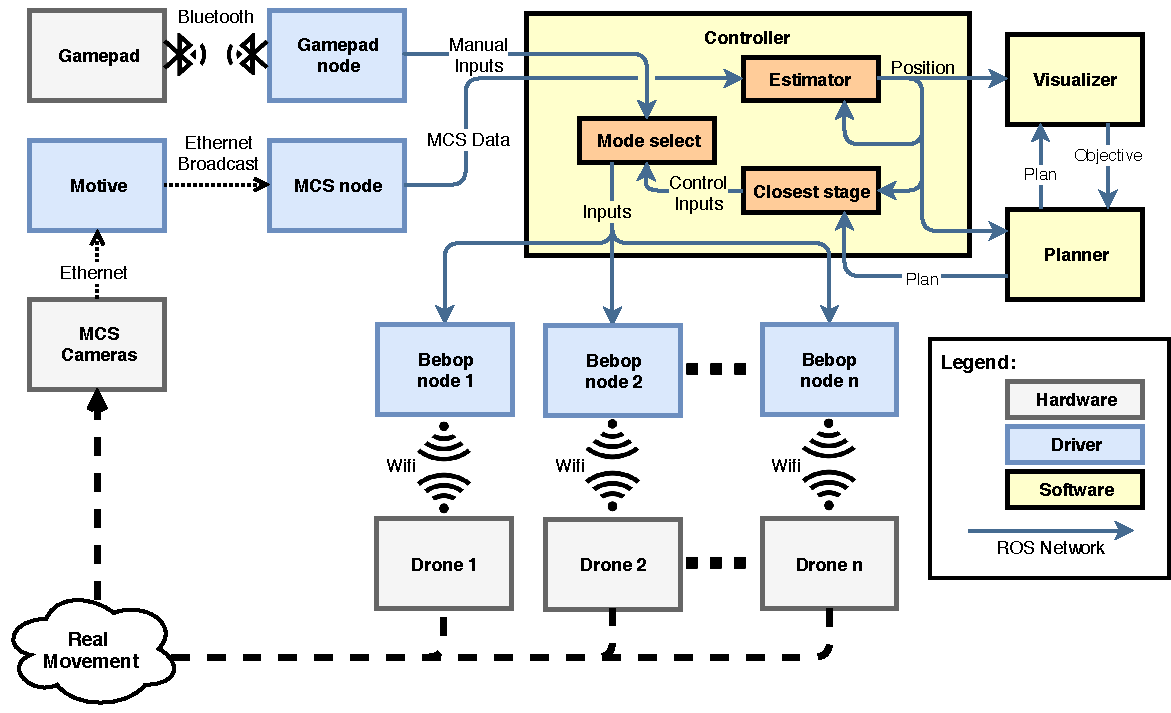
\includegraphics[width=1\linewidth]{Figures/Communications}
	\caption{Communications schematic}
	\label{fig::communications}
\end{figure}

\subsection{Rosbags}
One of the advantages of using \ac{ROS} for data communication is that we can use rosbags. Rosbags let us record all data into a file and then replay it. Even more, we can parse these files using \code{MATLAB} and analyze the data as we wish.

\section{Visualizer}
\label{sect::visualizer}
The visualizer is a \ac{GUI} created with \code{MATLAB}. A screenshot of the \ac{GUI} can be seen in \cref{fig::visualizer}. Through this interface we can:
\begin{itemize}
	\item See a representation of the system state and the obstacles in three dimensions.
		\subitem The drones are represented in black. 
		\subitem The wires are seen as blue lines.
		\subitem The payload is drawn as a red dot.
		\subitem The obstacles are displayed as gray boxes.
		\subitem The ellipsoids around the obstacle are shown as a brown surface.
		\subitem The planned trajectories of the drones are displayed as pink lines.
		\subitem The planned trajectory of the payload is shown as a dashed pink line.
		\subitem The current objective is drawn as a pink dot.
	\item See the numeric values of the current system state and inputs.
	\item Restart the simulated movement of the obstacles.
	\item Change the objective.
	\item Load and replay recorded data from a rosbag file.
\end{itemize}

\begin{figure}
	\centering
	\makebox[\textwidth][c]{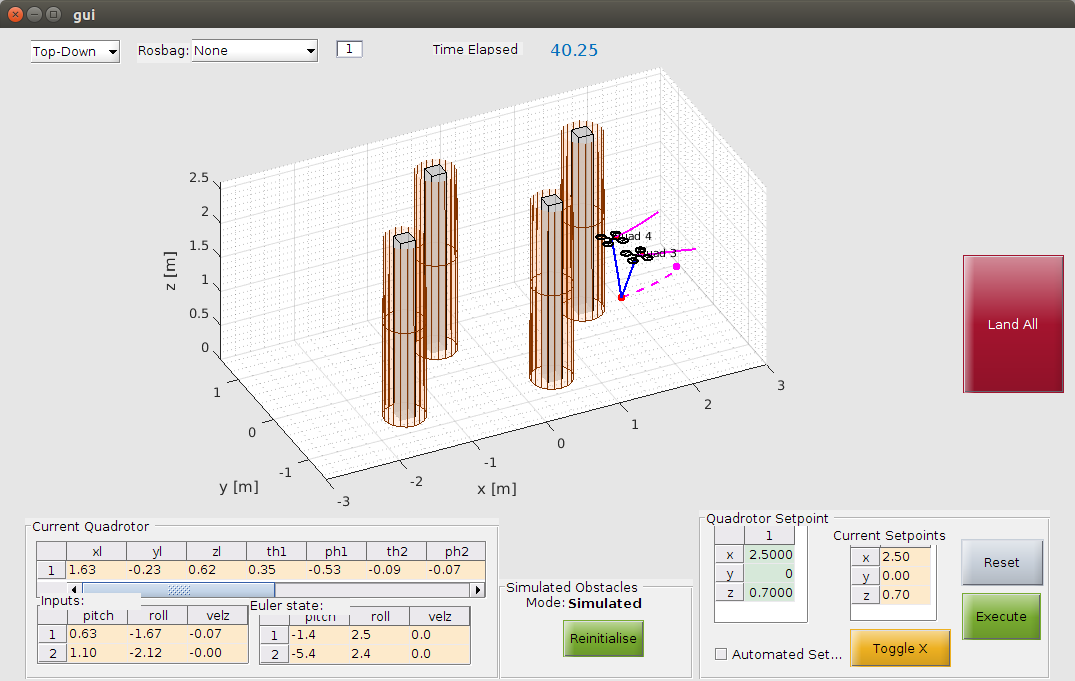
\includegraphics[width=1.2\linewidth]{Figures/visualizer}}
	\caption{Screenshot of the visualizer \ac{GUI}}
	\label{fig::visualizer}
\end{figure} 

